% Created 2025-11-09 søn 21:23
% Intended LaTeX compiler: pdflatex
\documentclass[smaller, aspectratio=169]{beamer}
\usepackage[utf8]{inputenc}
\usepackage[T1]{fontenc}
\usepackage{graphicx}
\usepackage{longtable}
\usepackage{wrapfig}
\usepackage{rotating}
\usepackage[normalem]{ulem}
\usepackage{amsmath}
\usepackage{amssymb}
\usepackage{capt-of}
\usepackage{hyperref}
\usepackage{natbib, dsfont, pgfpages, tikz,amssymb, amsmath,xcolor}
\bibliographystyle{abbrvnat}
\setbeamertemplate{footline}[frame number]
\beamertemplatenavigationsymbolsempty
\usepackage{appendixnumberbeamer}
\setbeamercolor{gray}{bg=white!90!black}
\setbeamertemplate{itemize items}{$\circ$}
\definecolor{bblue}{rgb}{0.2,0.2,0.7}
\newcommand{\E}{{\ensuremath{\mathop{{\mathbb{E}}}}}}
\newcommand{\R}{\mathbb{R}}
\newcommand{\N}{\mathbb{N}}
\newcommand{\blank}{\makebox[1ex]{\textbf{$\cdot$}}}
\newcommand\independent{\protect\mathpalette{\protect\independenT}{\perp}}
\def\independenT#1#2{\mathrel{\rlap{$#1#2$}\mkern2mu{#1#2}}}
\renewcommand{\phi}{\varphi}
\renewcommand{\epsilon}{\varepsilon}
\newcommand*\diff{\mathop{}\!\mathrm{d}}
\newcommand{\weakly}{\rightsquigarrow}
\newcommand\smallO{\textit{o}}
\newcommand\bigO{\textit{O}}
\newcommand{\midd}{\; \middle|\;}
\newcommand{\1}{\mathds{1}}
\usepackage{ifthen} %% Empirical process with default argument
\newcommand{\G}[2][n]{{\ensuremath{\mathbb{G}_{#1}}{\left[#2\right]}}}
\DeclareMathOperator*{\argmin}{\arg\!\min}
\DeclareMathOperator*{\argmax}{\arg\!\max}
\newcommand{\V}{\mathrm{Var}} % variance
\newcommand{\eqd}{\stackrel{d}{=}} % equality in distribution
\newcommand{\arrow}[1]{\xrightarrow{\; {#1} \;}}
\newcommand{\arrowP}{\xrightarrow{\; P \;}} % convergence in probability
\newcommand{\KL}{\ensuremath{D_{\mathrm{KL}}}}
\newcommand{\leb}{\lambda} % the Lebesgue measure
\DeclareMathOperator{\TT}{\Psi} % target parameter
\newcommand{\empmeas}{\ensuremath{\mathbb{P}_n}} % empirical measure
\usetheme{default}
\author{Anders Munch}
\date{\today}
\title{HTE reading group}
\begin{document}

\maketitle

\begin{frame}[label={sec:orge5199cf}]{Paper}
\begin{block}{Generic machine learning inference on heterogeneous treatment effects in randomized experiments, with an application to immunization in India}
by Victor Chernozhukov, Mert Demirer, Esther Duflo, and Iván
Fernández-Val

\hfill

\vfill

775 citations on Google Scholar. 
\end{block}
\end{frame}

\begin{frame}[label={sec:org2f2f31c}]{Focus}
Conceptual focus.

\vfill

Less focus on the actual estimators and the technical requirements for
their validity.

\vfill

More focus on the interpretation of the estimand and null hypotheses
that these estimators targets.
\end{frame}

\begin{frame}[label={sec:orgc953463}]{Major points}
Target \textbf{features} of CATE

\vfill

Estimands that depend on machine learning \textbf{proxies} of CATE

\vfill

\color{gray}{Insights on best \textbf{approximations} of CATE (in \textbf{RCT}s!)}
\end{frame}



\begin{frame}[label={sec:orgcb97bcc}]{Motivation}
Estimation of CATE (or even low-dimensional features of it) is too
hard.

\vfill

\begin{quotation} %% 
Without some form of sparsity, it is hard, if not impossible, to
obtain consistent estimators of [CATE]. \ldots{} One fundamental reason is
that ML methods might not even produce consistent estimators of [CATE]
in high dimensional settings. \ldots{} Hence, generic ML estimators cannot
be regarded as consistent, unless further assumptions are
made. Examples of such assumptions include structured forms of linear
and non-linear sparsity and super-smoothness. The problem of obtaining
uniformly valid inference on [CATE] using generic ML methods is even
more difficult.

In this paper, we take an agnostic view. We neither rely on any
sparsity or low-complexity assumptions to make the ML estimators
consistent, nor impose other stronger conditions to make ``traditional''
confidence intervals valid. We simply treat ML as providing proxy
predictors for the objects of interest. (p.8)
\end{quotation}
\end{frame}


\begin{frame}[label={sec:orgda49040}]{Some notation and setup}
Potential outcomes \( Y(0) \) and \( Y(1) \), binary treatment
indicator \( D \), and high-dimensional covariate vector \( Z \).

\vfill

Main causal functions (identified through standard assumptions) are
\begin{equation*}
  b_0(z)
  =
  {\color{gray}b_P(z)= \;} 
  \E{\left[ Y(0) \mid Z = z \right]}
  = \E{\left[ Y \mid D=0, Z = z \right]}
\end{equation*}
and the CATE function
\begin{equation*}
  s_0(z)
  =
  {\color{gray}s_P(z) = \;} 
  \E{\left[ Y(1) - Y(0)\mid Z = z \right]}
  = \E{\left[ Y(0) \mid Z = z \right]} - \E{\left[ Y \mid D=0, Z = z \right]}
\end{equation*}

\vfill

The propensity score
\begin{equation*}
  p(z) = P(D=1 \mid Z) = P(D=1 \mid Z_1)
\end{equation*}
is \textbf{known}, i.e., RCT setting. 


\vfill

\( B(z) = B_a(z) = B(z; \text{Data}) \) and
\( S(z) = S_a(z) = S(z; \text{Data}) \) denote \textbf{machine
  learning proxies} for \( b_P \) and \( s_P \).
\end{frame}


\begin{frame}[label={sec:orgd521204}]{Stage 1 \small (p.9)}
\begin{center}
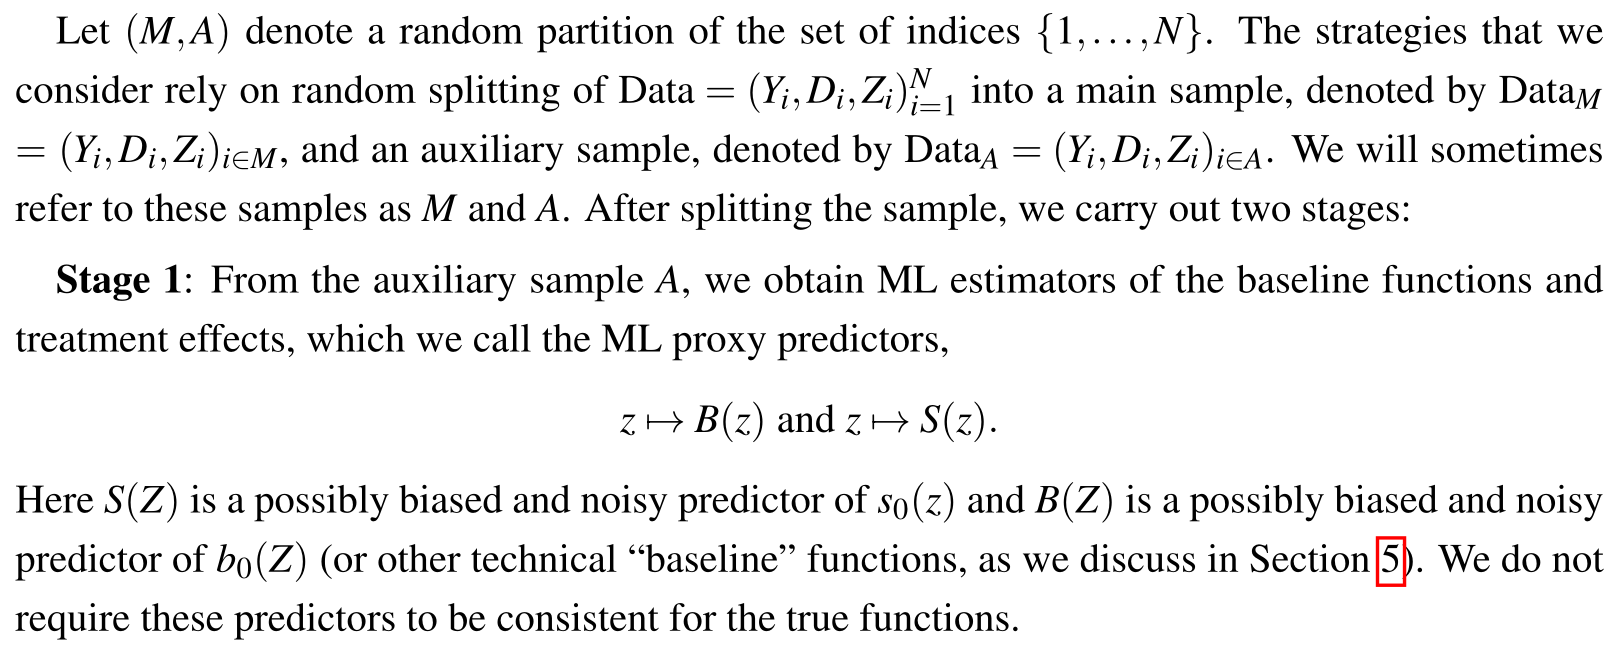
\includegraphics[width=1\textwidth]{./paper-ss/ss-p9-step1.png}
\end{center}
\end{frame}


\begin{frame}[label={sec:orgec5cff9}]{Stage 2 \small (p.9)}
\begin{center}
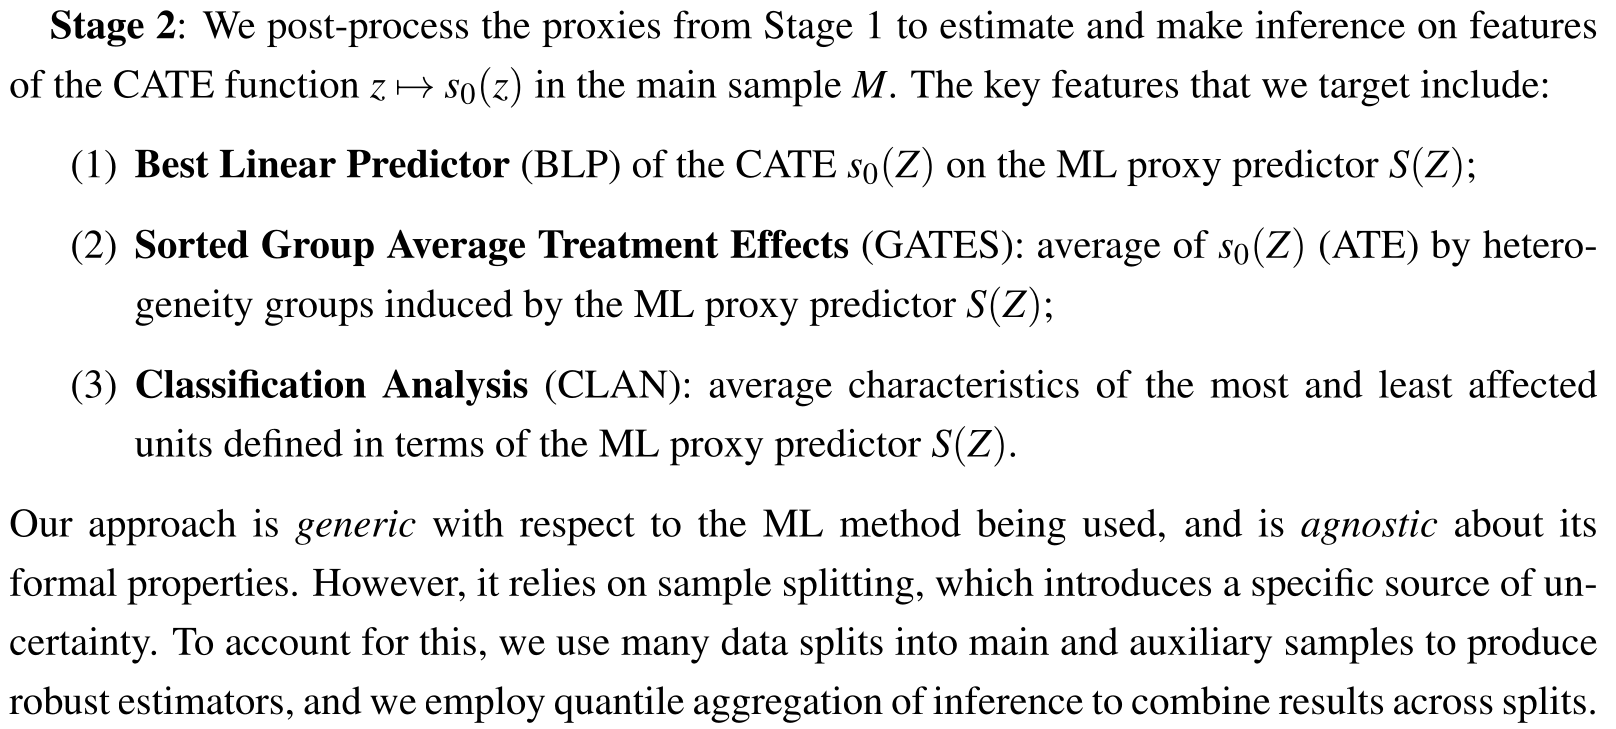
\includegraphics[width=1\textwidth]{./paper-ss/ss-p9-step2.png}
\end{center}
\end{frame}


\begin{frame}[label={sec:orgf291cfc}]{Summary of the proposal}
Split data into main and auxiliary samples.

\vfill

\begin{description}
\item[{Stage 1}] Fit complex ML algorithms for estimating \(b_0\) and \(s_0\) in the auxiliary sample, obtaining the proxies \(B\) and \(S\).
\end{description}
\vfill

\begin{description}
\item[{Stage 2}] Consider \(B\) and \(S\) as fixed functions and
estimate some low-dimensional feature of them and the true CATE \(s_0\)  in
the main sample.
\end{description}

\vfill

Repeat and base inference on quantiles obtained across different
splits into main and auxiliary samples.
\end{frame}


\begin{frame}[label={sec:org3bcfe8c}]{Conditional (data-adaptive) estimands \small (p.12)}
\begin{center}
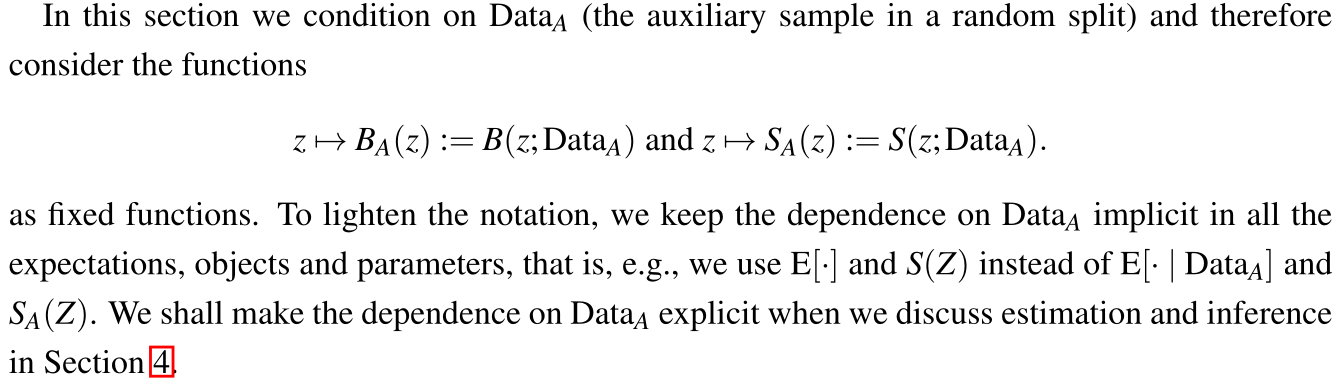
\includegraphics[width=1\textwidth]{./paper-ss/ss-p12-cond-data.png}
\end{center}
\end{frame}



\begin{frame}[label={sec:org453accb}]{Example of feature: Best Linear Prediction (BLP) \small (compare p.12)}
\begin{definition}[BLP]
The best linear predictor of \( s_P(Z) \) by \( S(Z) = s_A(Z) = S(Z ; \text{Data}_A) \) is the
solution to
\begin{equation*}
  \min_{b_1 \in \R, b_2 \in \R} \E_P{\left[ (s_{P}(Z) - b_1 - b_2 S(Z ;
      \text{Data}_A))^2 \mid \text{Data}_A \right]},
\end{equation*}
which, if exists, is defined as
\begin{equation*}
  \text{BLP}_P[s_{P}(Z) \mid S(Z; \text{Data}_A)] := \beta_1 + \beta_2
  (S(Z; \text{Data}_A) 
  -\E_P{\left[ S(Z; \text{Data}_A) \mid \text{Data}_A \right]}),
\end{equation*}
where \( \beta_1 = \E_P{\left[ s_P(Z) \right]} \) and
\( \beta_2 = \text{Cov}_P[s_P(Z), S(Z; \text{Data}_A) \mid
\text{Data}_A]/\text{Var}_P[S(Z; \text{Data}_A) \mid \text{Data}_A]
\).
\end{definition}

\begin{block}{}
I write \(s_P = s_0\) and \(\E_P= \E\) to make it clear that the
``true'' expectation \(\E\) means the expectation under \(P\)
according to which the ``true'' CATE \(s_0\) is defined.
\end{block}
\end{frame}


\begin{frame}[label={sec:org1872d02}]{Why conditioning on data?}
They are discussing \textbf{two} things to address the \emph{``fundamental
impossibilities in non-parametric inference [of CATE estimation]''}
(p.3).

\vfill

\begin{description}
\item[{Firstly:}] Target low-dimensional features of CATE, e.g., BLP,
GATE, CLAN.
\end{description}

\vfill

Why not stop here?

\begin{itemize}
\item[$\rightarrow$] Would require that the CATE function can be
  approximated fast enough, typically at a rate which should be \(
  \smallO_P(n^{-1/4}) \).
\item[$\rightarrow$] This is unrealistic in truly high-dimensional settings
(i.e., realistic finite-sample scenario). 
\end{itemize}

\vfill

\begin{description}
\item[{Secondly:}] Target low-dimensional features of
\textbf{data-dependent proxies} of CATE and make inference
\textbf{conditional on data}.
\end{description}

\vfill

\begin{beamercolorbox}[rounded=true]{gray}
\centering Trading unachievable rate-convergence criteria for
post-selection inference interpretations.
\end{beamercolorbox}
\end{frame}




\begin{frame}[label={sec:orgfa782db}]{Definition and interpretation of the estimand \small (p.21)}
\begin{center}
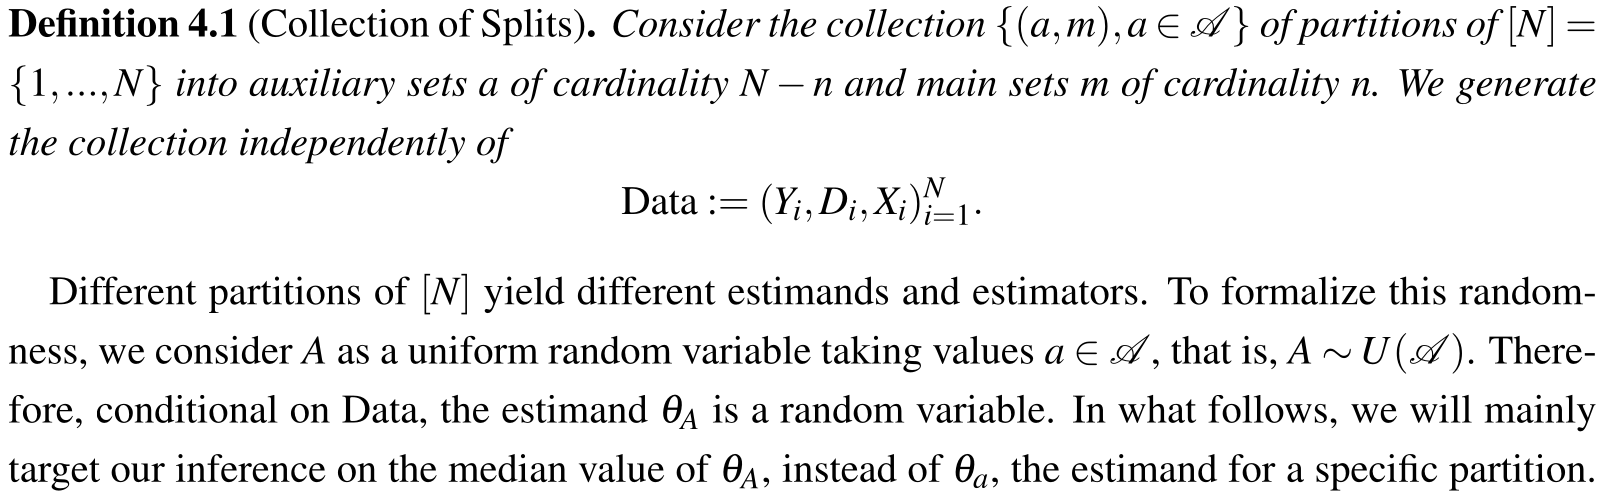
\includegraphics[width=1\textwidth]{./paper-ss/ss-p21-median-random-est.png}
\end{center}
\end{frame}


\begin{frame}[label={sec:org271a8f7}]{Definition and interpretation of the estimand -- my attempt}
Define the data-dependent parameter $\theta(P, \text{Data}_a)$ as
\begin{equation*}
  \theta(P; S, \text{Data}_a) = \text{BLP}_P[s_0(Z) \mid S(Z; \text{Data}_a)].
\end{equation*}
The data-dependent ``median'' parameter $\theta_{\text{M}}(P,
\text{Data})$ is defined as
\begin{equation*}
  \theta_{\text{M}}(P; S, \text{Data})
  = \text{Median}(\theta(P; S, \text{Data}_A) \mid \text{Data})
  = \text{Median}_{A \sim U(\mathcal{A})}(\theta(P; S, \text{Data}_A) \mid \text{Data}).
\end{equation*}

\vfill

Would the parameter \( \theta(P; S, \text{Data}) \) be more
interesting? Or  \( \E{[\theta(P; S, \text{Data})]} \)?

\vfill

Would we expect the parameter \( \theta_{\text{M}}(P; \text{Data}) \) to
be close to \( \theta(P; \text{Data}) \) or \( \E{[\theta(P; S, \text{Data})]} \)?

\vfill

Can we relate the interpretation of this to the type of performance measures we get from cross-validation?
\end{frame}


\begin{frame}[label={sec:orga48cbb4}]{Interpretation of null hypothesis}
\begin{center}
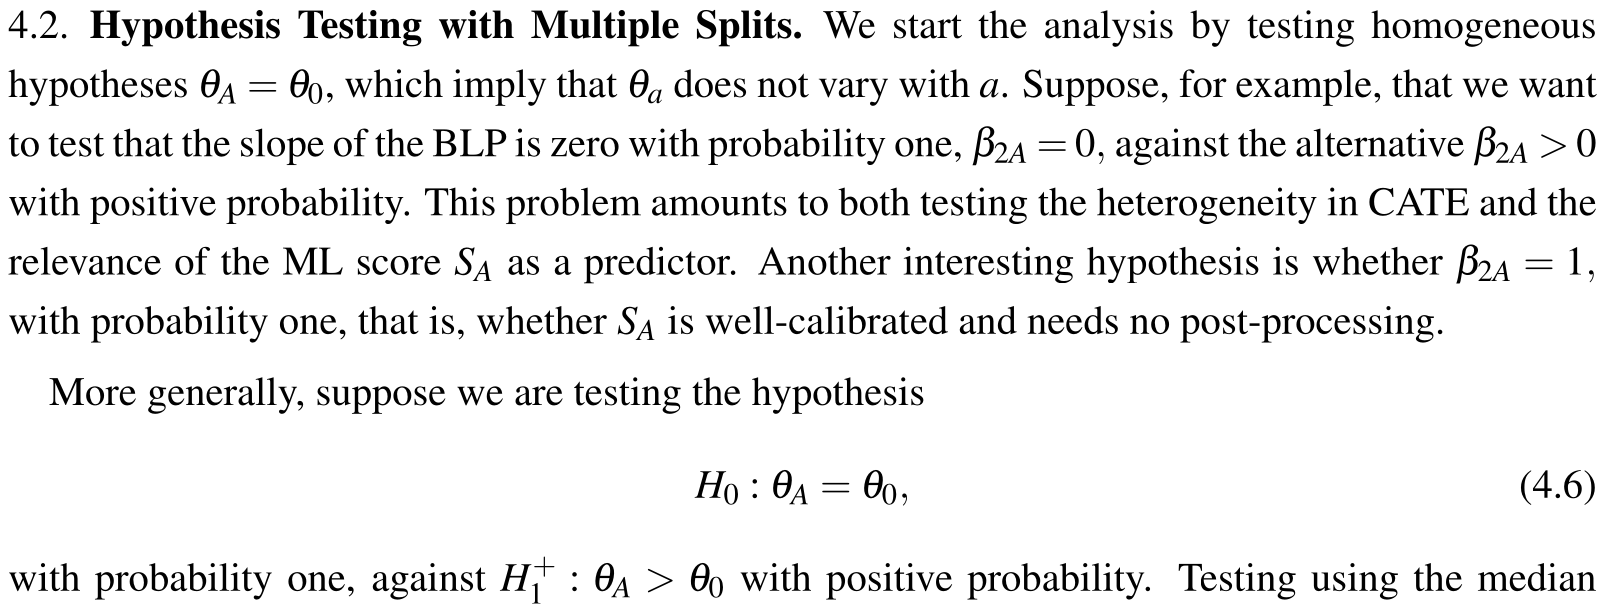
\includegraphics[width=1\textwidth]{./paper-ss/ss-p23-null-hypo.png}
\end{center}
\end{frame}


\begin{frame}[label={sec:org222659a}]{Applied analysis}
Immunization (vaccination?) of children i North India (against
measles?).
\end{frame}

\begin{frame}[label={sec:org8debfe4}]{Interpretation of results}
\begin{center}
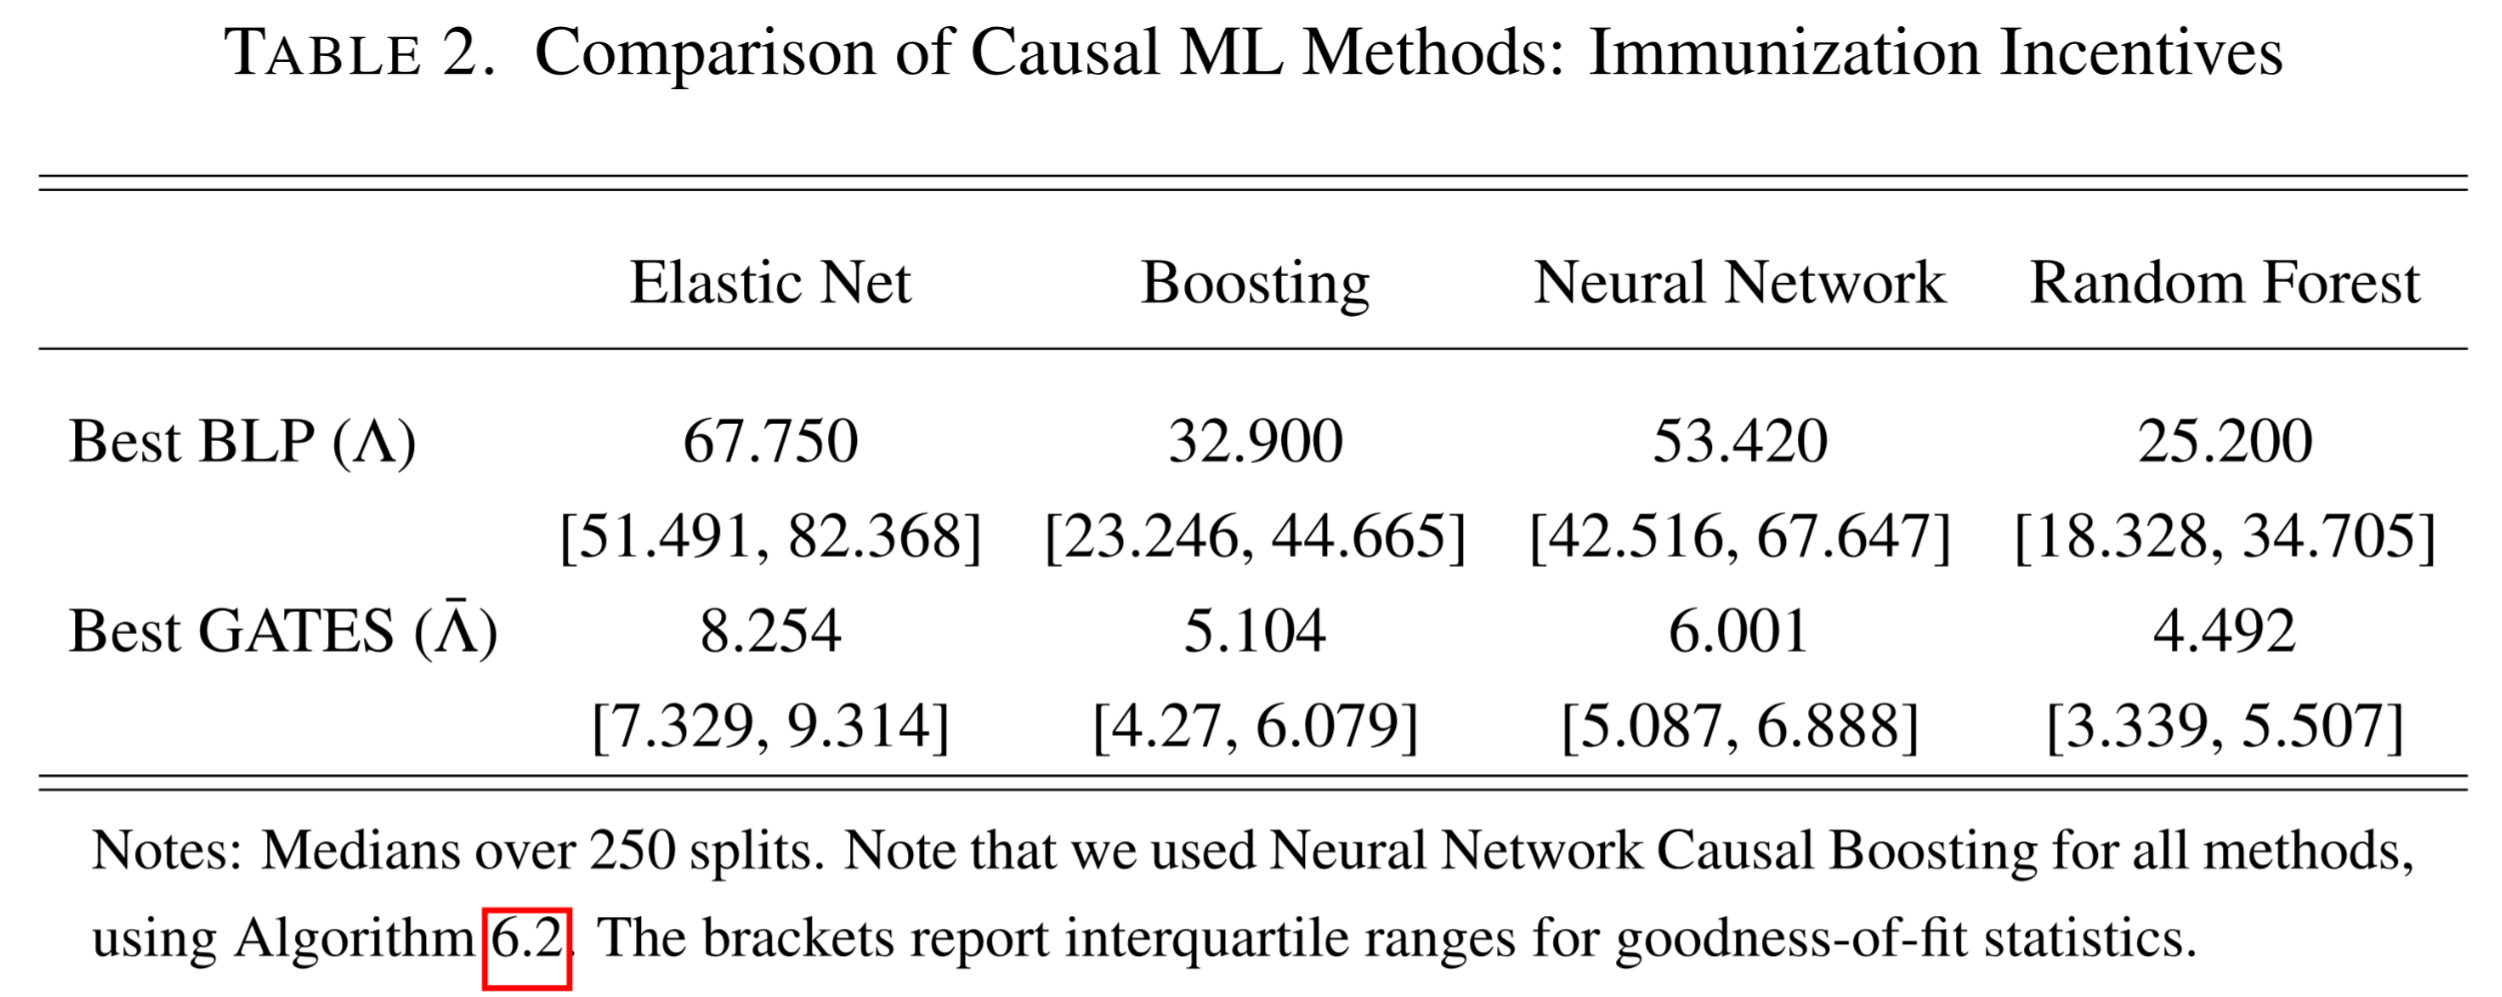
\includegraphics[width=1\textwidth]{./paper-ss/ss-table2.png}
\end{center}
\end{frame}


\begin{frame}[label={sec:org3f7fc47}]{Interpretation of results}
\begin{center}
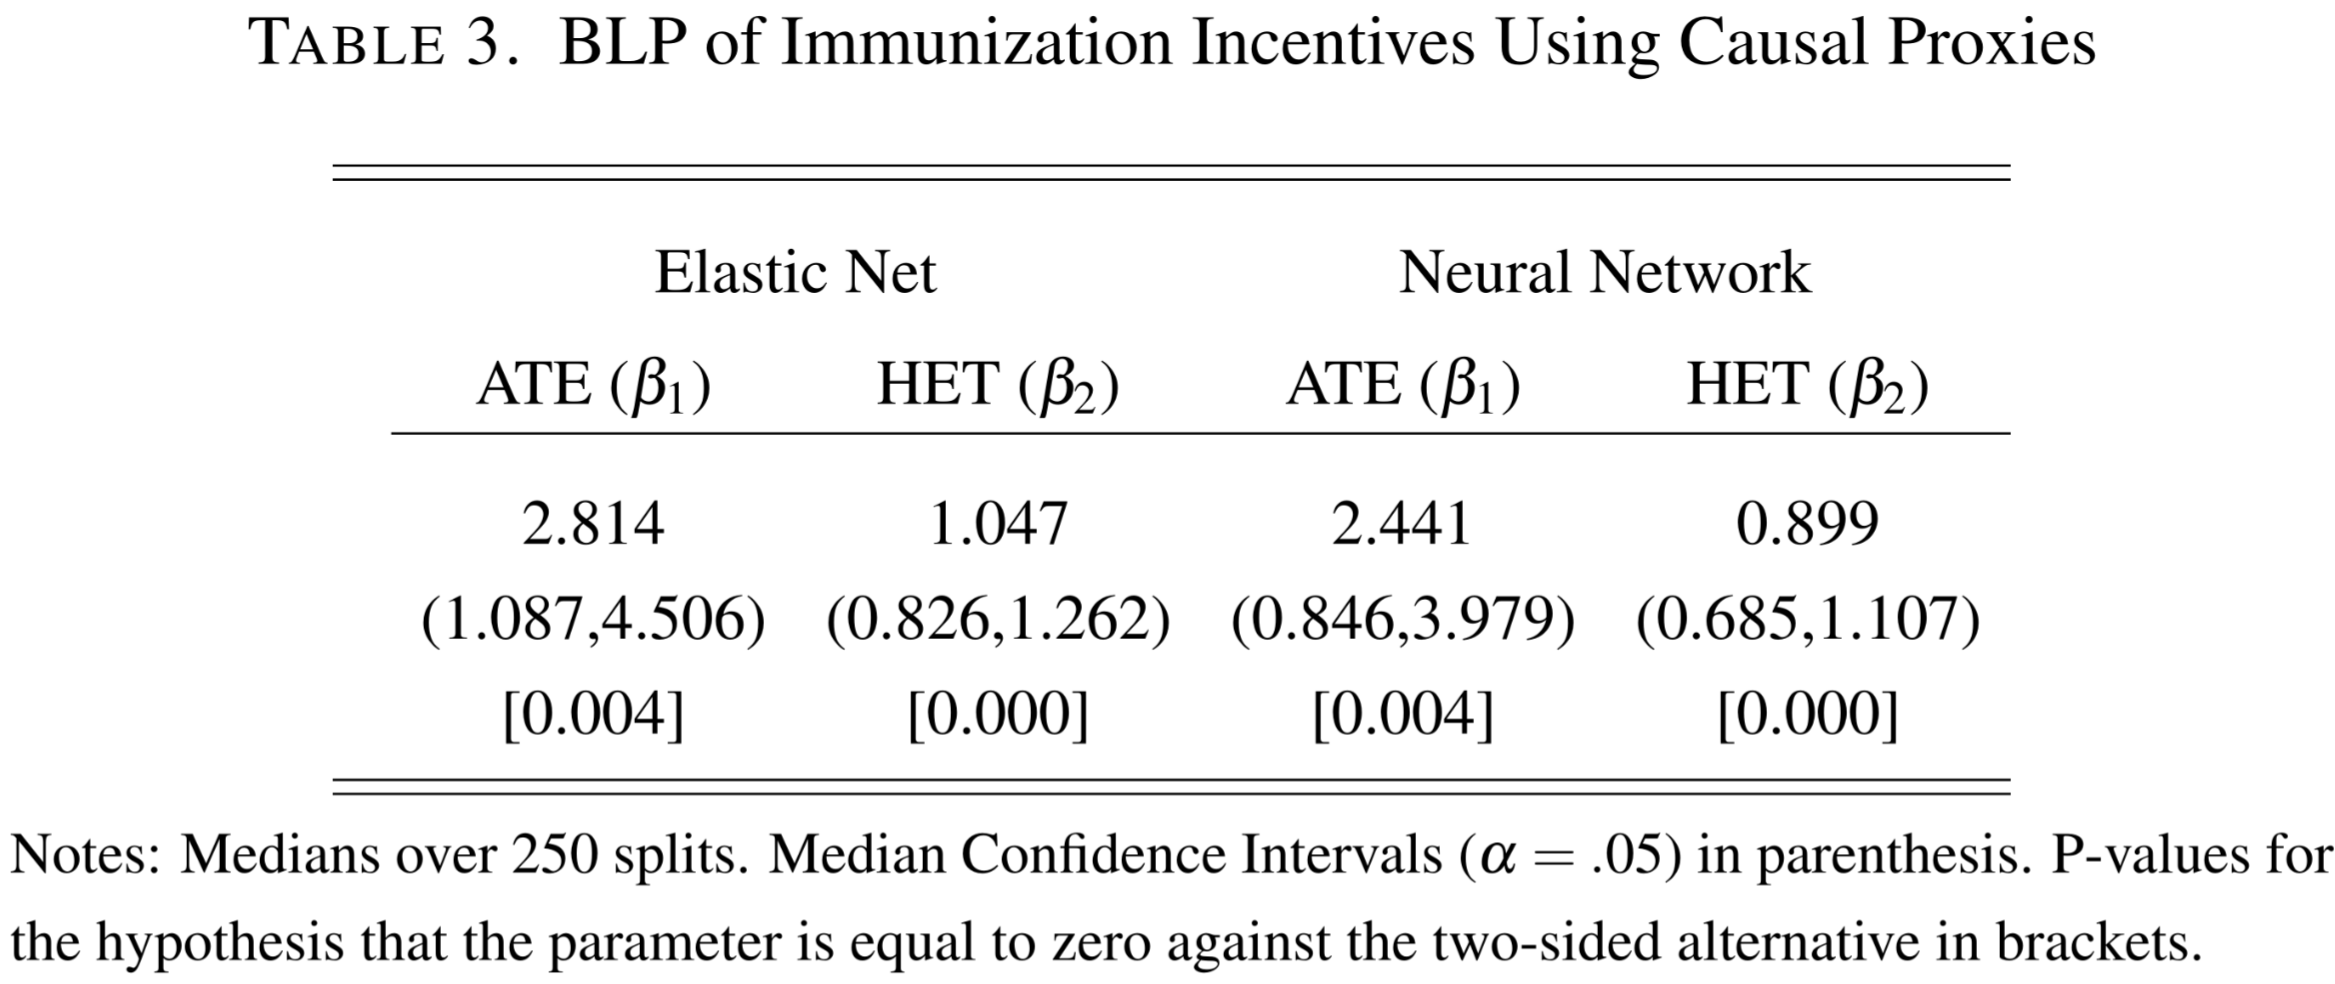
\includegraphics[width=.7\textwidth]{./paper-ss/ss-table3.png}
\end{center}

\begin{center}
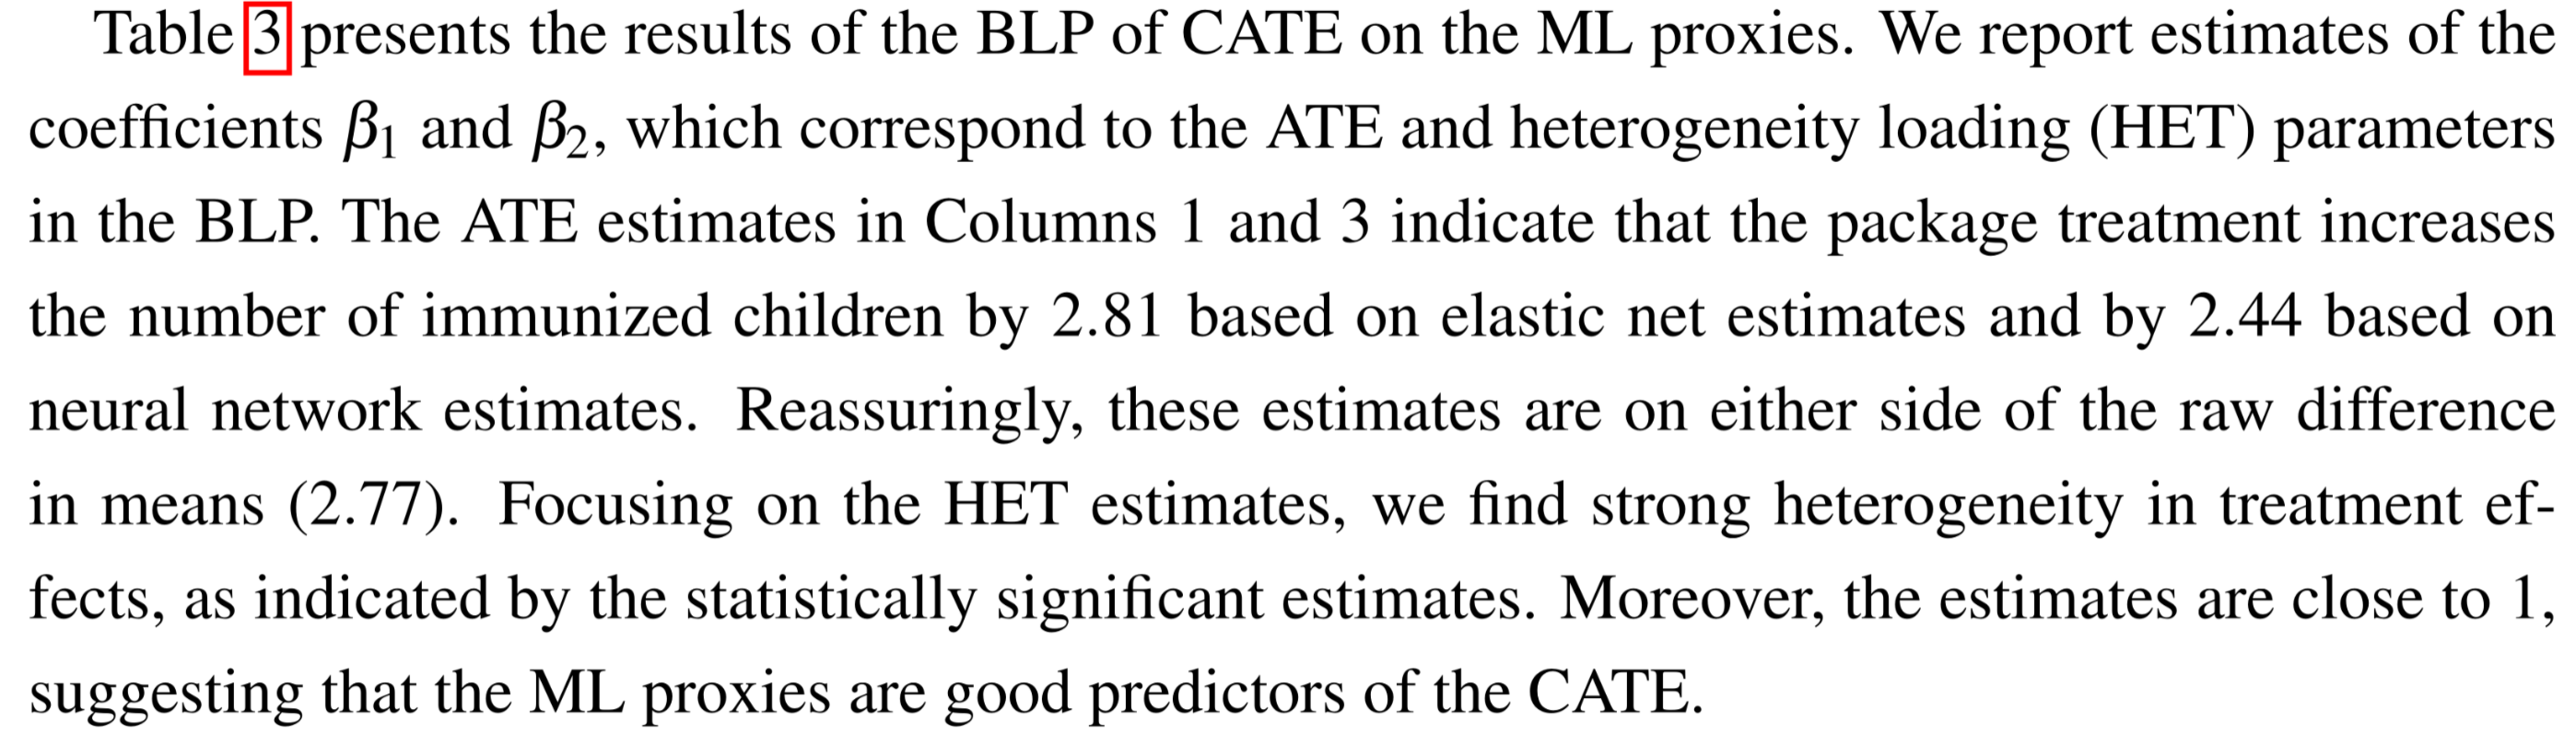
\includegraphics[width=.9\textwidth]{./paper-ss/ss-table3-decr.png}
\end{center}
\end{frame}


\begin{frame}[label={sec:org1778ada}]{Addendum: Best approximation of CATE (in RCTs)}
Getting the best approximation of CATE \(s_0\) based on the proxy \(S\) is not just OLS -- need to use weight based on the propensity
score.

\vfill

Alternatives for building causal learners of CATE.

\vfill

These tricks only seem to work in an RCT setting(?). So comparison
with existing method, which may be developed for observational
settings, are perhaps not fair. 
\end{frame}
\end{document}
